\documentclass[12pt, letterpaper]{article}

% Create metadata
\title{Chapter 1 exercises from The Algorithm Design Manual}
\author{Chas Keithan}
\date{August 28, 2023}

\usepackage{preamble}

%start document
\begin{document}
\maketitle
\section{Exercises}
\subsection{[3] Show that $a+b$ can be less than $min(a,b)$}
    Let $a: -2$ and $b: -3$
    \begin{align*}
        min(a, b) =& min(-2,-3) = -3\\
        a + b =& -2 + -3 = -5\\
        -5 <& -3
    \end{align*}
\subsection{[3] Show that $a*b$ can be less than $min(a,b)$}
    Let $a: -1$ and $b: 2$
    \begin{align*}
        min(a ,b) =& min(-1,2) = -1\\
        a * b =& -1 * 2 = -2\\
        -2 <& -1
    \end{align*}
\subsection{[5] Design/draw a road network with two points $a$ and $b$ such that the fastest route between $a$ and $b$ is not the shortest route.}
    \begin{center}
        \begin{tikzpicture}
            \node[location] at (0,0) (a) {$a$};
            \node[location] (b) at (2,0) {$b$}
                edge [<-, bend right, above] node {5mph} (a)
                edge [<-,below] node {1mph} (a); 
        \end{tikzpicture}
    \end{center}
\subsection{[5] Design/draw a road network with two points $a$ and $b$ such that the shortest route between $a$ and $b$ is not the route with the fewest turns.}
    \begin{center}
        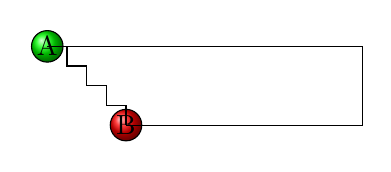
\begin{tikzpicture}
            \draw [ball color=green,fill] (0,0) circle [radius=0.2] node [black] {A};
            \draw [ball color=red,fill] (1,-1) circle [radius = 0.2] node [black] {B};
            \draw(0,0) to (4,0) to (4,-1) to (1,-1);
            \draw(0,0) to (0.25,0) to (0.25,-0.25) to (0.5,-0.25) to (0.5,-0.5) to (0.75,-0.5) to (0.75,-0.75) to (1,-0.75) to (1,-1);
        \end{tikzpicture}
    \end{center}
\subsection{[4] Given a set of integers $S = {s_1,s_2,\dots,s_n}$, and a target number $T$, find a subset of $S$ which adds up exactly to $T$\\Find counterexamples to each of the following algorithms for the knapsack problem.}
    \begin{enumerate}[label=\alph*)]
        \item{Put the elements of $SW$ in the knapsack in left to right order if they fit, i.e. the first-fit algorithm}
        \item{Put the elements of $S$ in the knapsack from smallest to largest, i.e. the best-fit algorithm}
        \item{Put the elements of $S$ in the knapsack from largest to smallest}
    \end{enumerate}
    Let $S = \{1,3,5,7,9\}$ and $T = 11$
    \begin{enumerate}[label=\alph*)]
        \item{
            \[\{1\}=1<11\]
            \[\{1,3\}=4<11\]
            \[\{1,3,5\}=9<11\]
            \[\{1,3,5,7\}=16>11\]
            \[\{1,3,5,9\}=18>11\]
            but \[\{1,3,7\} == 11\]
        }
        \item{
            \[\{1\}=1<11\]
            \[\{1,3\}=4<11\]
            \[\{1,3,5\}=9<11\]
            \[\{1,3,5,7\}=16>11\]
            \[\{1,3,5,9\}=18>11\]
            but \[\{1,3,7\} == 11\]
        }
        \item{
            \[\{9\}=9<11\]
            \[\{9,7\}=12>11\]
            \[\{9,5\}=14>11\]
            \[\{9,3\}=12>11\]
            \[\{9,1\}=10<11\]
            but \[\{1,3,7\} == 11\]
        }
    \end{enumerate}
\subsection{[6] The \emph{set cover problem}: given a set of subsets $S_1,\dots,S_m$ of the universal set $U = \{1,\dots,n\}$, find the smallest subset of subsets $T \subset S$ such that $\cup_{t_i \in T} t_i = U$.\\Find a counterexample for the following algorithm: Select the largest subset for the cover, and then delete all its elements from the universal set. Repeat by adding the subset containing the largest number of uncovered elements until all are covered.}
    Let $U = \{0,1,2,3,4,5,6,7,8,9\}$ and 
    \[S_1 = \{1,3,5,7,9\}\]
    \[S_2 = \{1,2,3,4,5\}\]
    \[S_3 = \{0,6,7,8,9\}\]

    \begin{enumerate}
        \item{Since they all have 5 elements of the universal set, we can start with any of them. The first makes logical sense, so we will start with $S_1$: \[T = \{S_1\}\]\[U \rightarrow \{0,2,4,6,8\}\]$S_2$ now has 2 in $U$ and $S_3$ now has 3.}
        \item{Using $S_3$ next: \[T = \{S_1,S_3\}\]\[U \rightarrow \{2,4\}\]$S_2$ still has 2 in $U$}
        \item{Finally add in $S_2$ for a subset of subsets that covers the universal set.\\Compare this subset to $S_2$ and $S_3$\[S_2 + S_3 == U \quad \&\& \quad T_{{S_2},{S_3}} \subset T_{{S_1},{S_2},{S_3}}\]}
    \end{enumerate}

\subsection{[3] Prove the correctness of the following recursive algorithm to multiply two natural numbers, for all integer constants $c \geq 2$.}
    \begin{lstlisting}[language=Python]
    def multiply(y,z):
        if z==0:
            return 0
        else:
            multiply(c*y, floor(z/c)) + y * (z%c))
    \end{lstlisting}
    Obviously, the case of $z=0$ is correct as it returns $0$. We can also show that $z=1$ is similarly as trivial since $z < c$ and will return \[multiply(cy,0) + yz \quad \Rightarrow \quad yz\].

    We will assume that the condition holds true for all $z \leq n-1$ and prove that it holds for $z=n$

    Let $z =n= cx$ where $x$ is an integer.

    \begin{align}\setcounter{equation}{0}
        &multiply(y, cx)\\
        &multiply(cy, x) + y(cx~mod~c)\\
        &multiply(cy, x) + 0\\
        &cyx~\Rightarrow~ycx~\Rightarrow~yz
    \end{align}

    Now we will let $z = n = cx - a$ where $x$ is still an integer and $a<c$.
\subsection{[3] Prove the correctness of the following algorithm for evaluating a polynomial.\\$P(x)~=~a_nx^n~+~a_{n-1}x^{n-1}~+~\dots~+~a_1x~+~a_0$}
    \begin{lstlisting}[language=Python]
    def horner(A,x):
        p = A_n
        for i in range(len(A_n)-1, 0, -1):
            p = p*x + A_n[i]
        return p
    \end{lstlisting}
    Obviously, when $A_0 = \{a_0\}$ the loop will not run and it will simply return $a_0$.\\
    Likewise, when $A_1 = \{a_0,a_1\}$ the loop will run once and return $a_1x + a_0$ as expected.\\
    We will assume the function works for $A_{n-1}$ and prove it for $A_n$.
    \begin{align}\setcounter{equation}{0}
            &a_nx + A_{n-1}\\
            &(a_nx^n + a_{n-1}x^{n-1}
    \end{align}
\subsection{Scratch Stuff Below}
\lstinputlisting[language=c++]{test.cpp}
\section{exercises}
This is a test

\end{document}
